\documentclass[crop=false, class=book]{standalone}

%impostazioni lingua
\usepackage[T1]{fontenc}
\usepackage[utf8]{inputenc}
\usepackage[english,italian]{babel}

\usepackage[dvipsnames]{xcolor}
\usepackage{listings}

\lstdefinelanguage{Kotlin}{
	comment=[l]{//},
	commentstyle={\color{gray}\ttfamily},
	emph={[1]first, firstOrNull, forEach, lazy, map, mapNotNull, println},
	emphstyle={[1]\color{OrangeRed}},
	identifierstyle=\color{black},
	keywords={!in, !is, abstract, actual, annotation, as, as?, break, by, catch, class, companion, const, constructor, continue, crossinline, data, delegate, do, dynamic, else, enum, expect, external, false, field, file, final, finally, for, fun, get, if, import, in, infix, init, inline, inner, interface, internal, is, lateinit, noinline, null, object, open, operator, out, override, package, param, private, property, protected, public, receiveris, reified, return, return@, sealed, set, setparam, super, suspend, tailrec, this, throw, true, try, typealias, typeof, val, var, vararg, when, where, while, it},
	keywordstyle={\color{NavyBlue}\bfseries},
	morecomment=[s]{/*}{*/},
	morestring=[b]",
	morestring=[s]{"""*}{*"""},
	ndkeywords={@Deprecated, @JvmField, @JvmName, @JvmOverloads, @JvmStatic, @JvmSynthetic, Array, Byte, Double, Float, Int, Integer, Iterable, Long, Runnable, Short, String, Any, Unit, Nothing, Config, LightEstimationMode, CameraConfigFilter, CameraConfig, FacingDirection, AugmentedFaceMode, AugmentedFace, TrackingState, RegionType, CloudAnchorMode,AugmentedImageDatabase, BitmapFactory, Session, InstantPlacementMode, File, Uri, RecordingConfig },
	ndkeywordstyle={\color{BurntOrange}\bfseries},
	sensitive=true,
	stringstyle={\color{ForestGreen}\ttfamily},
	emph={[2]FRONT,MESH3D,ENVIRONMENTAL\_HDR,AMBIENT\_INTENSITY, DISABLED,FOREHEAD\_LEFT,FOREHEAD\_RIGHT,NOSE\_TIP, TRACKING, ENABLED, LOCAL\_Y\_UP},
	emphstyle={[2]\color{Purple}\ttfamily},
}

\definecolor{lightgrey}{RGB}{230,237,244}

\lstset{
	basicstyle=\scriptsize\sffamily\color{black},
	backgroundcolor=\color{lightgrey},
	frame=single,
	numbers=left,
	numbersep=5pt,
	numberstyle=\tiny\color{gray},
	showspaces=false,
	showstringspaces=false,
	tabsize=1,
	texcl=true,
	captionpos=b,
	breaklines=true
}




%sistema i margini
\usepackage{geometry}
\geometry{a4paper,top=2.2cm,bottom=2.2cm,left=3cm,right=3cm, heightrounded}

%interlinea 1.5
\usepackage{setspace}
\onehalfspacing

%gestione delle testatine
\usepackage{fancyhdr}
\pagestyle{fancy}
\lhead{}
\chead{}
\rhead{Titolo}
\lfoot{}
\cfoot{\thepage}
\rfoot{}
\renewcommand{\headrulewidth}{0.4pt}

%formattazione titoli paragrafo
\usepackage{titlesec}
\titleformat{\chapter}[block]{\normalfont\huge\bfseries}{\thechapter.}{0.7em}{\huge}

%pacchetti per i riferimenti in bibliografia
\usepackage[autostyle,italian=guillemets]{csquotes}
\usepackage[style=numeric,citestyle=numeric-comp,backend=biber]{biblatex}

%risorsa che contiene la bibliografia
\addbibresource{./../bibliografia.bib}

\usepackage{lipsum}
\usepackage{graphicx}
\usepackage[italian]{varioref}
\usepackage{copyrightbox}
\usepackage{subfig}


\begin{document}

	\chapter{User Interaction}
	ARCore utilizza la tecnologia \textit{ray casting} per permettere all'utente di posizionare un oggetto nella scena corrente 	in un punto fissato. Quando lo schermo del telefono viene toccato o viene compiuta qualche altra interazione, 					viene proiettato un raggio nella visuale del mondo della fotocamera che può intersecare un preciso punto o piani 				geometrici. ARCore permette di ricavare un elenco dei risultati delle intersezioni con la geometria della scena rilevata 		attraverso gli hitTest. Solitamente il primo risultato è quello più significativo perchè si riferisce all'intersezione più 		vicina al dispositivo.
	
	\begin{figure}
			\centering
			\copyrightbox[b]{
				\subfloat[][\emph{}]
				{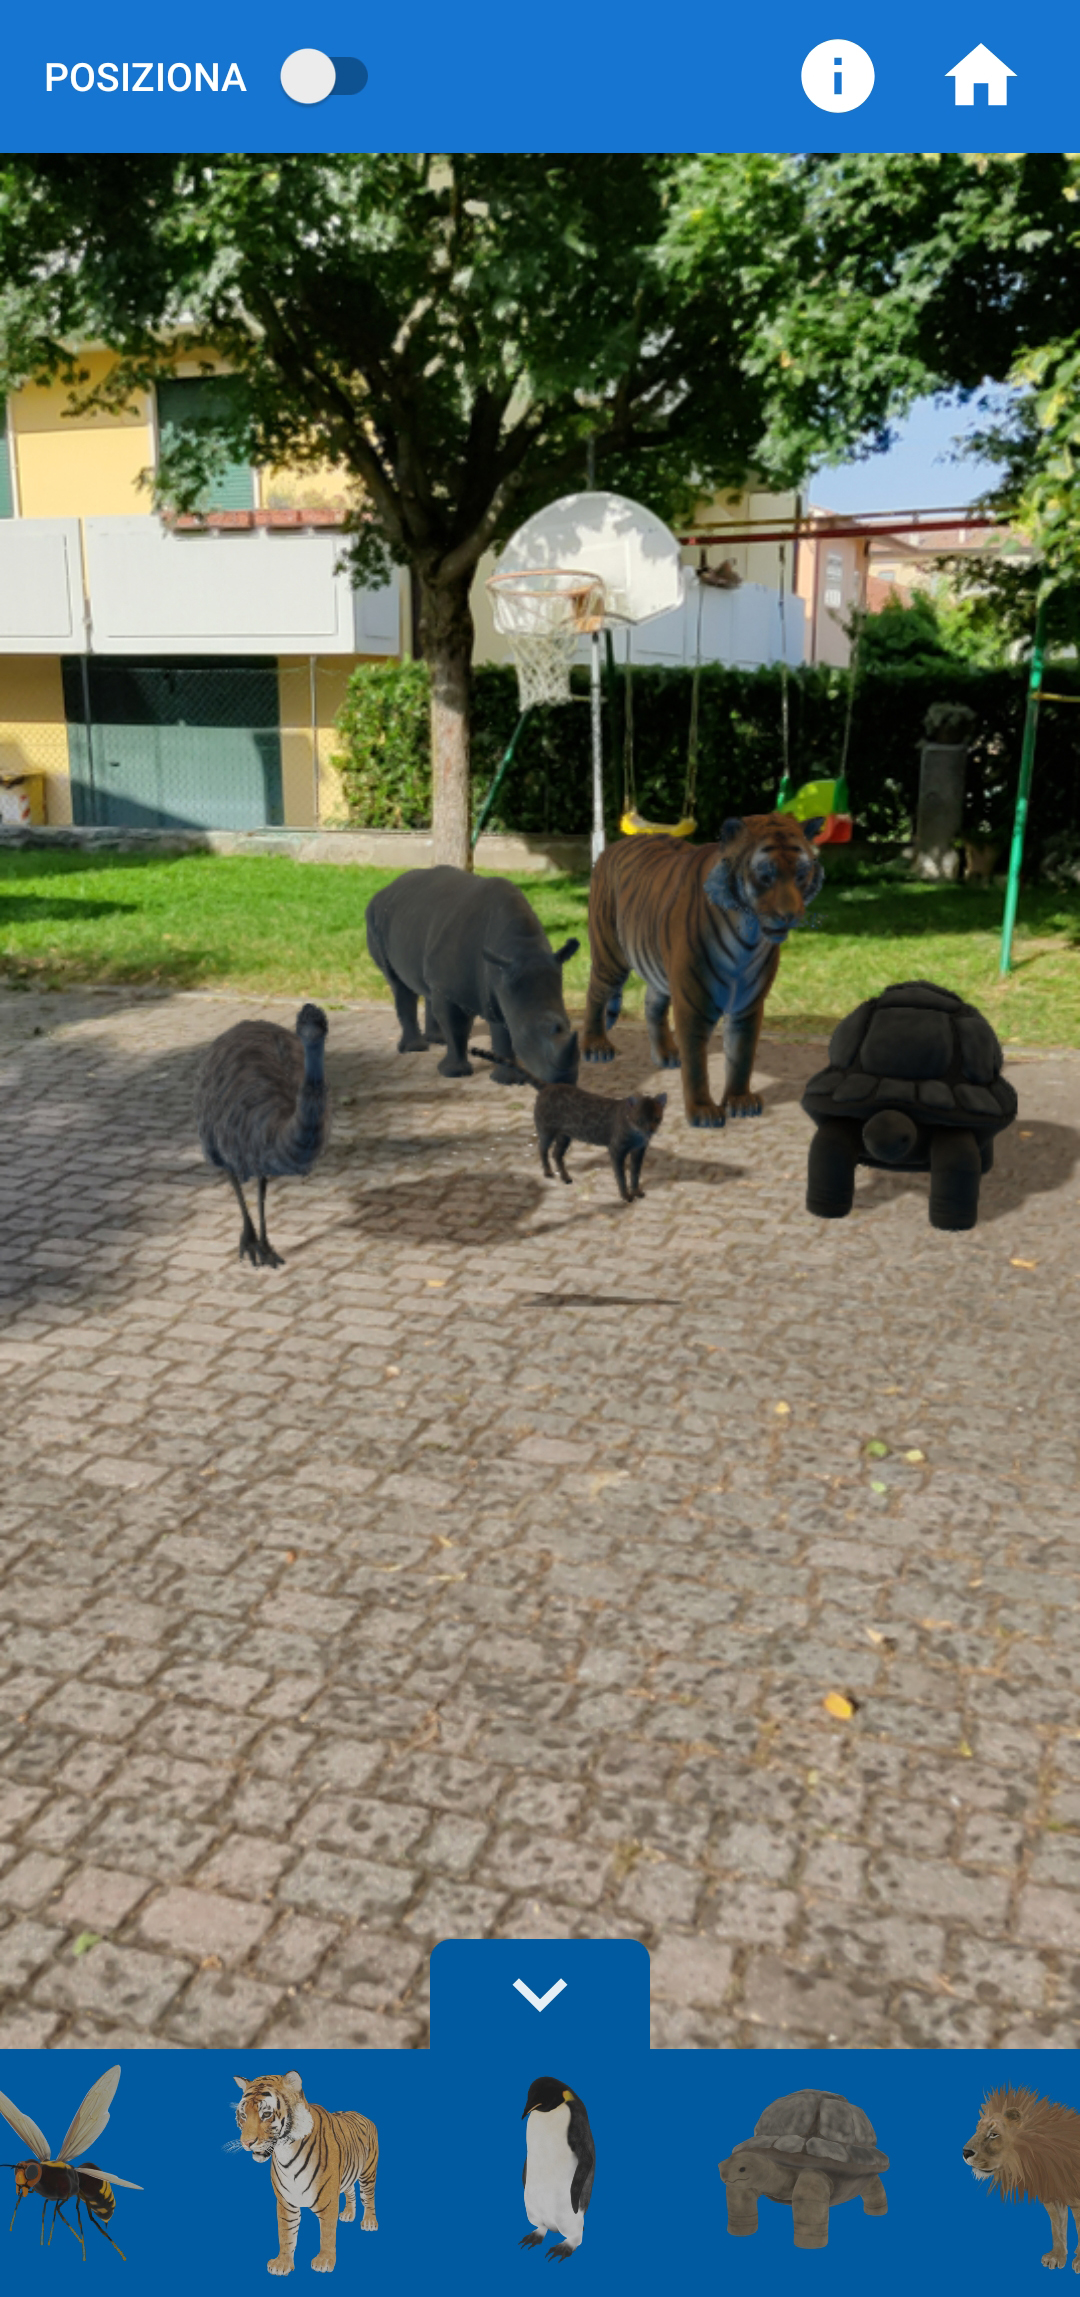
\includegraphics[width=0.3\textwidth]{../../resources/images/UserInteraction/Animals1.jpg}}  \quad,
				\subfloat[][\emph{}]
				{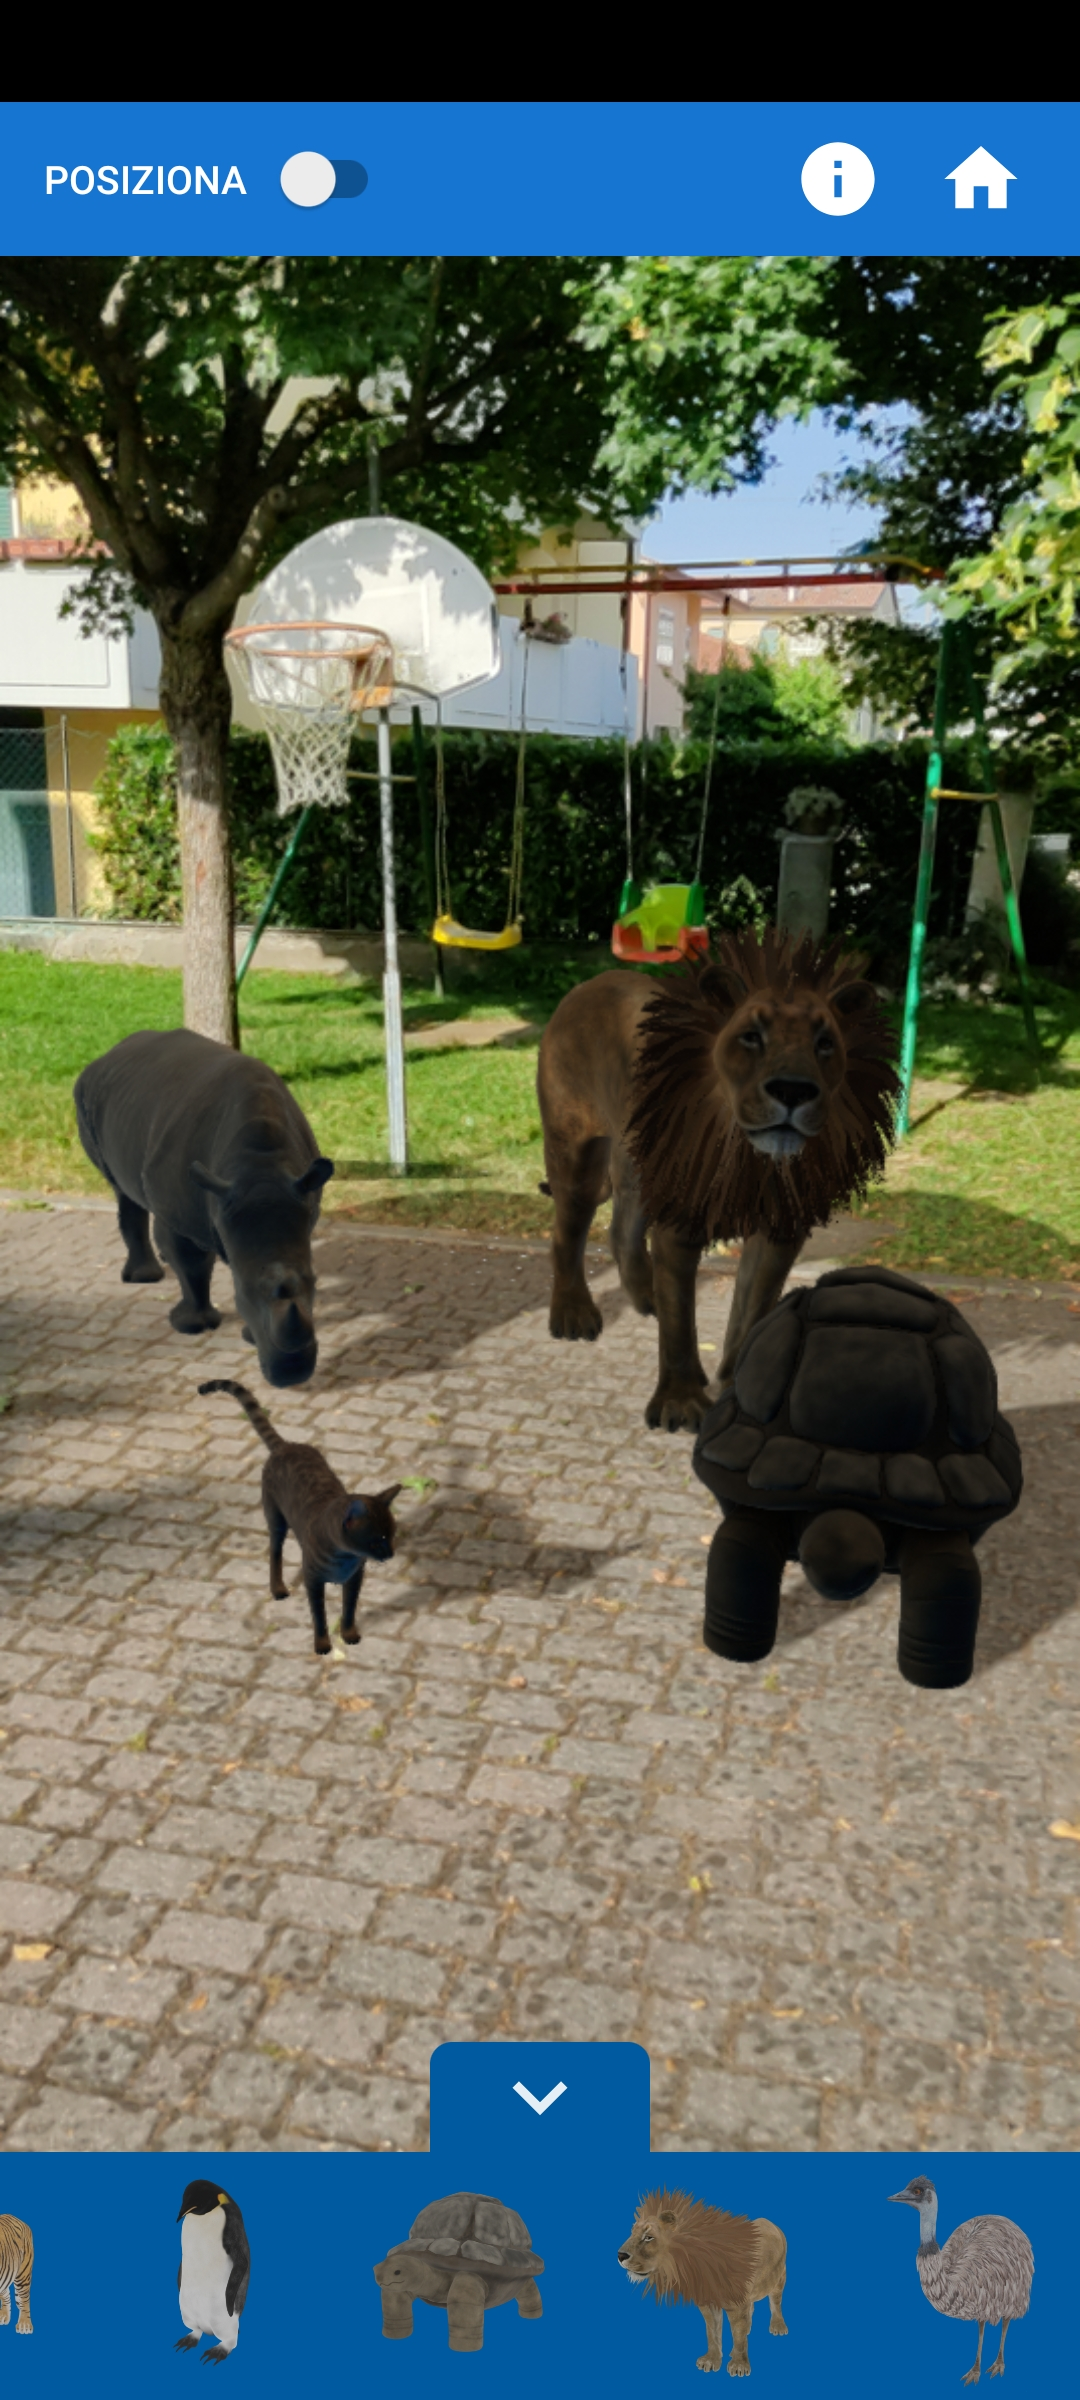
\includegraphics[width=0.3\textwidth]{../../resources/images/UserInteraction/Animals2.jpg}} \quad,
			}{Fonte: \url{}}	
			\caption{Esempio di molteplici hitTest su un piano in Plane Detection}
			\label{fig:pet_img}
	\end{figure}
	
	\begin{flushleft}
		Un potenziale test per stimare le performance dell'interazione con l'utente potrebbe consistere nel posizionare un 				numero notevole di oggetti virtuali nella scena ed 	esaminare se le performance diminuiscono con 								l'incremento del numero di oggetti.  Si potrebbe scoprire se esiste una soglia di numero di oggetti  per la 					quale l'applicazione si arresta. Si consiglia di eliminare anchor inutili per evitare che le performance 						diminuiscano notevolmente.
	\end{flushleft}
			
	
\end{document}